\documentclass[a4paper,11pt]{article}
\usepackage{graphicx}
\usepackage{mathrsfs}
\usepackage{amssymb,amsfonts,amsmath}
\usepackage{multirow}
\usepackage{epsfig}
\usepackage{subfigure}

\def\pdfshellescape{1}
\usepackage{epstopdf}

\usepackage{color}
\usepackage{float}
%opening
\title{Course2012 Assignment 5}
\author{Institute of Computing Technology, \\
                       Chinese Academy of Sciences, Beijing, China }

\begin{document}

\maketitle

Notice:\\\\
1. Due Dec. 21, 2012 for the course in S301, Teaching Building\\
\qquad Due Dec. 26, 2011 for the course in Conference Hall, ICT Building\\
2. Please send your answer in hard copy.\\
3. You can choose two problems from Problem 1-7\\
4. You can present your answer in English or in Chinese.

\section{Prime and Dual}
Suppose that we are given a linear program $L$ in standard form, and suppose that for both $L$ and the dual of $L$, the basic solutions associated with the initial slack forms are feasible. Show that the optimal objective value of $L$ is 0.

\section{Linear-Inequality Feasibility}
Given a set of $m$ linear inequalities on $n$ variables $x_1$, $x_2$,...,$x_n$, the {\bf linear-inequality feasibility problem} asks if there is a setting of the variables that simultaneously satisfies each of the inequalities.\\\\
{\bf a.} Show that if we have an algorithm for linear programming, we can use it to solve the linear-inequality feasibility problem. The number of variables and constraints that you use in the linear-grogramming problem should be polynomial in $n$ and $m$.\\\\
{\bf b.} Show that if we have an algorithm for the linear-inequality feasibility problem, we can use it to solve a linear-programming problem. The number of variables and linear inequalities that you use in the linear-inequality feasibility problem should be polynomial in $n$ and $m$, the number of variables and constraints in the linear programming.

%\section{Linear Programming}
%Suppose that $Y$ is a random variable taking on one of $n$ known values:
%$$a_1,a_2,...,a_n.$$
%Suppose we know that $Y$ either has distribution $p$ given by
%$$\mathbb{P}(Y=a_j)=p_j$$
%or it has distribution $q$ given by
%$$\mathbb{P}(Y=a_j)=q_j.$$
%Of course, the numbers $p_j$, $j=1,2,...,n$ are nonnegative and sum to one. The same is true for the $q_j$'s. Based on a single observation of $Y$, we wish to guess whether it has distribution $p$ or distribution $q$. That is, for each possible outcome $a_j$, we will assert with probability $x_j$ that the distribution is $p$ and with probability $1-x_j$ that the distribution is $q$. We wish to determine the probabilities $x_j,j=1,2,...,n$, such that the probability of saying the distribution is $p$ when in fact it is $q$ has probability no larger than $\beta$, where $\beta$ is some small positive value (such as 0.5). Furthermore, given this constraint, we wish to maximize the probability that we say the distribution is $p$ when in fact it is $p$. Formulate this maximization problem as a linear programming problem.

\section{Linear Programming Modelling}
{\sc Integer Linear Programming Problem} is different from the classic Linear Programming Problem that some extra constraints such as 
$$x_i\ is\ an\ integer,\ for\ all\ i=1,2,...,n$$
are added.\\\\
A railway station has estimated that at least the following number of staff is needed in each four-hour interval throughout a standard 24-hour period and the salary per hour for every person during the different period:
\begin{center}
\begin{tabular}{c|c}
 Time Period & Staff Needed\\
\hline
5:00-9:00 & $S_1$\\
9:00-13:00 & $S_2$\\
13:00-17:00 & $S_3$\\
17:00-21:00 & $S_4$\\
21:00-1:00 & $S_5$\\
1:00-5:00 & $S_6$
\end{tabular}
\begin{tabular}{c|c}
 Time Period & Salary Per Hour For Every Person\\
\hline
0:00-8:00 & $C_1$\\
8:00-16:00 & $C_2$\\
16:00-24:00 & $C_3$
\end{tabular}
\end{center}
All staff works in 8-hour-shifts, which means every person will do continuous work for 8 hours. There are six possible shifts that start on the hour in the beginning of each 4-hour period in the table. Now if the railway station want to minimize the total salary paid in one day, please formulate this problem as an integer linear programming problem.

\section{Linear Programming Modelling}
{\sc $0$-$1$ Integer Programming Problem} is different from the classic Linear Programming Problem that some extra constraints such as 
$$x_i\in\{0,1\},\ for\ all\ i=1,2,...,n$$
are added.\\\\
There is an undirected graph $G$ with $n$ nodes. We use a matrix $M$ to denote that whether two nodes are connected by an edge. In other words, $M_{ij}$ is 1 if $i$ and $j$ are adjacent, and 0 otherwise. If you want to paint the nodes with some colors, such that any two adjacent nodes don't share the same color, and you try to use as less colors as possible, please formulate this problem as an integer linear programming problem (see the definition in Problem 4) or a 0-1 linear programming problem.

\section{Linear Programming Modelling}
In a directed acyclic graph, you can find no path which start from some node and stop at the same node. In this case, there are no Hamilton Cycle in this graph. In some practical problems, we will modify the conditions a little so as to find some approximate solutions. For example, the original target can be modifed to finding the minimum number of paths so that you're able to visit all nodes when you go through all these paths. The beginning and end of the paths are not restricted. In the following instance, the minimum number of paths is 2, and the paths are colored red.
\begin{figure}[H]
   \centering
   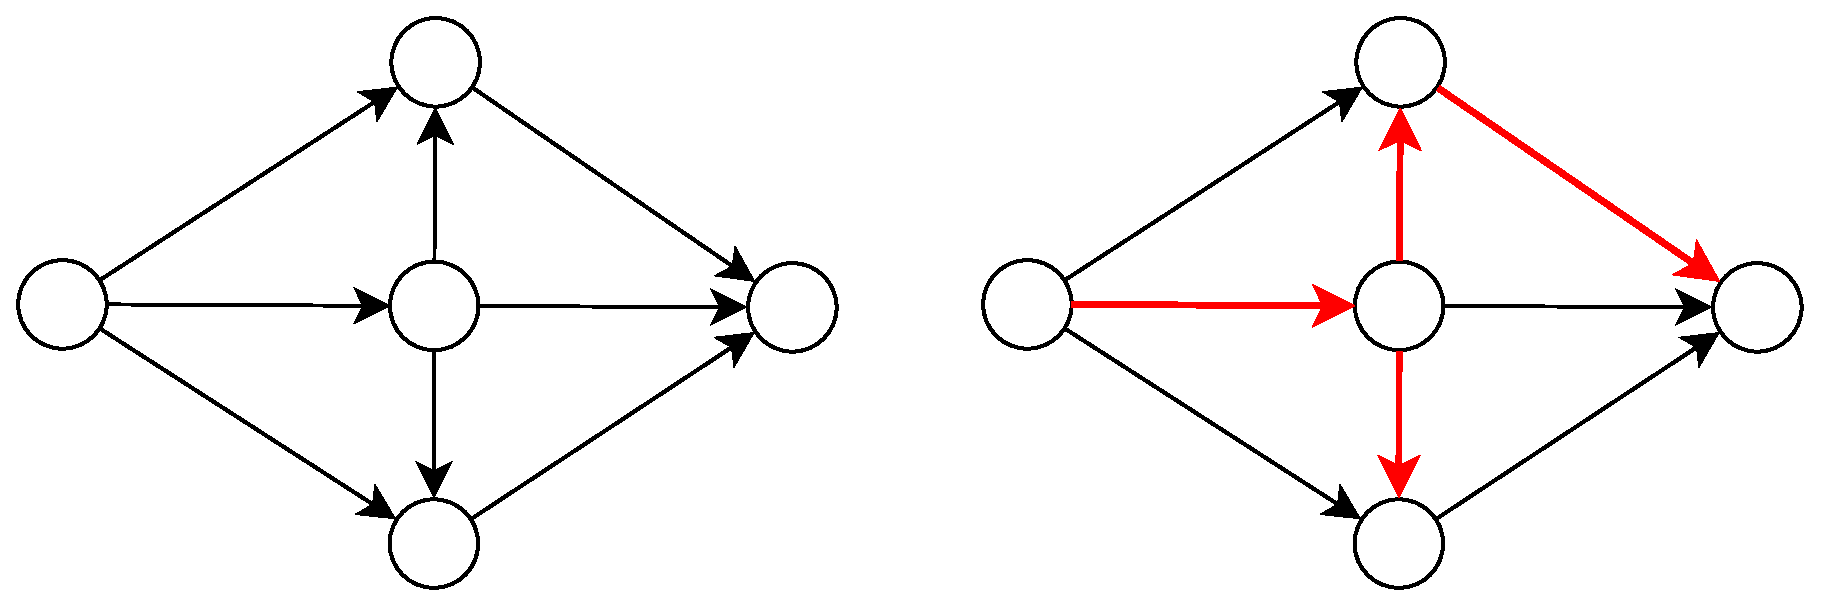
\includegraphics[width=2.8in]{minimum_paths.eps}
  \label{minimum_paths}
\end{figure}
Try to formulate this modified problem as a linear programming problem or an integer linear programming problem (see the definition in Problem 4) or a 0-1 linear programming problem (see the definition in Problem 5).\\\\
(Note: If you can't solve this problem, please tell us explicitly in your answer sheet; if you can solve it, please try to solve it in the answer sheet. Thank you very much.)
\section{Linear Programming Modelling}
Recall SMP($Stable\ Marriage\ Problem$), please try to fomulate SMP as a linear programming problem or an integer linear programming problem.

% \section{Linear Programming Modelling}
% FBI wants to send a very dangerous criminal from one prison to another. Just in case that the criminal be rescued, FBI decided to send several cars simultaneously to mislead his partners. The problem appears here: how to design the routes so as to arrange as many misleading cars as possible. Suppose all relative streets here are oneway streets. In this case, the problem can be transformed to finding as many paths as possible in a directed graph, while all these paths cannot share any node or edge except the starting point $s$ and the finishing point $t$. In the following example, the maximum number of paths is 3, and the available paths are colored red.
% \begin{figure}[H]
%    \centering
%    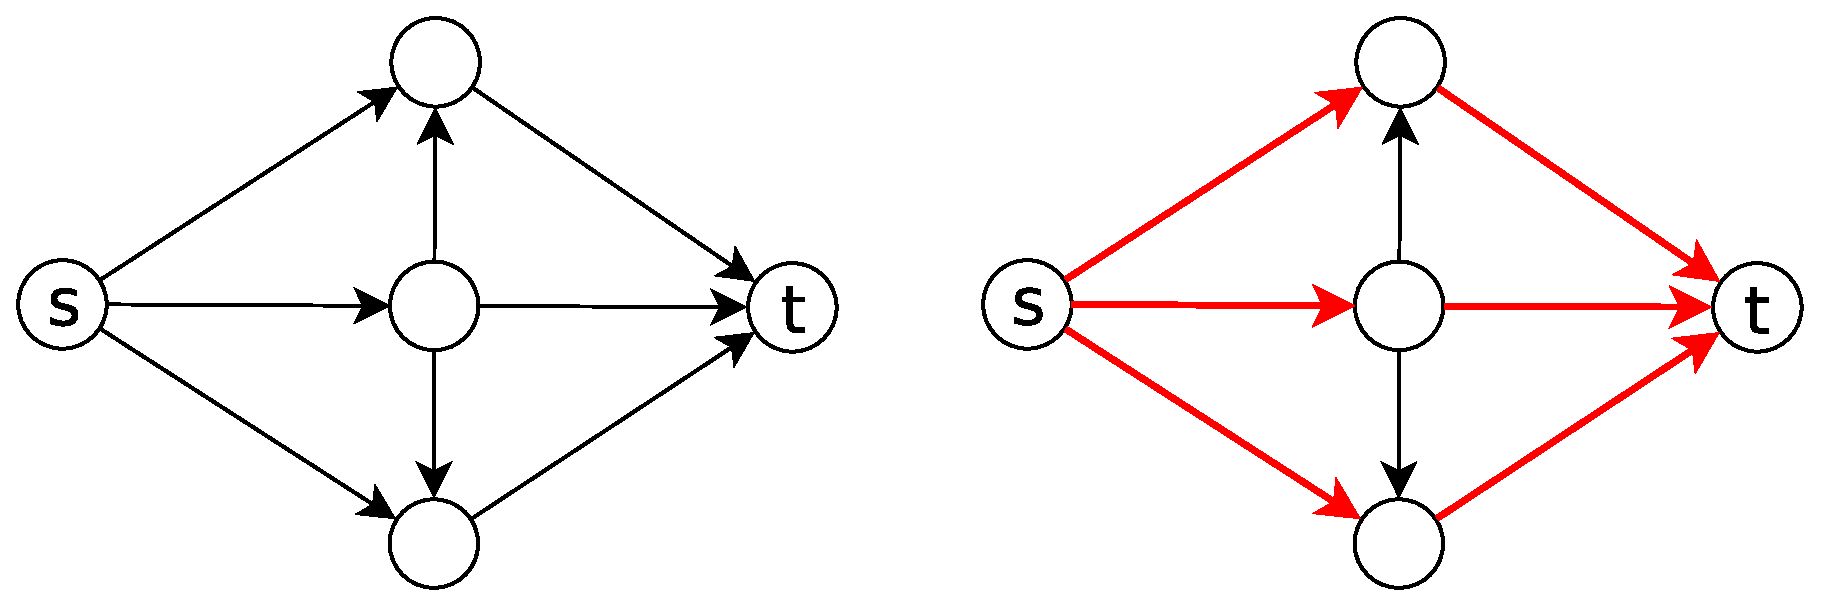
\includegraphics[width=2.8in]{maximum_paths.eps}
%   \label{maximum_paths}
% \end{figure}
% Try to formulate this problem as a linear programming problem or an integer linear programming problem (see the definition in Problem 4) or a 0-1 linear programming problem (see the definition in Problem 5).
\section{Linear Programming Modelling}
A factory plan to produce I \uppercase\expandafter{\romannumeral2} two products. The cost is as below:
\begin{center}
\begin{tabular}{p{2.5cm}|p{2.5cm}|p{2.5cm}|p{2.5cm}}
\hline 
 & I& II & \\
\hline
device & 1 & 2 &  8 \\ \hline
material A & 4 & 0 & 16kg\\ \hline
material B & 0 & 4 & 12kg\\ \hline 
\end{tabular}
\end{center}
The profit of product I is \$2, and the profit of product II is \$3. Please maximize the total profit.\\
(1)Try to formulate this problem as a linear programming problem.\\
(2)Try to give its dual and dual's dual. Explain the meaning of dual problem.\\
(3)Solve this problem with Simplex algorithm or Dual Simplex algorithm. Each iterate step should be written down in detail.\\

\end{document}
